\section{Architectural Design }
\label{sec:architectural_design}
% Begin Section

\subsection{System Architecture}
\label{sub:system_architecture}
% Begin SubSection
The overall architecture of our design follows the Pipe and Filter architecture. This serves as the overarching architecture composing of three subsystems with their own architectures, as shown in Table 1.

\begin{table}[h]
    \centering
    \renewcommand{\arraystretch}{1.5}
    \begin{tabular}{|c|p{8cm}|c|}
        \hline
        \textbf{Subsystem} & \textbf{Purpose} & \textbf{Architectural Style} \\
        \hline
        \textbf{Reader} & Reads the input from the user and converts it into the proper file format for the Identifier subsystem & Pipe and Filter \\
        \hline
        \textbf{Identifier} & Identifies the language using the input from the Reader subsystem & Blackboard \\
        \hline
        \textbf{Display (Facts)} & Obtains the proper facts of the identified language from the Identifier subsystem and displays it to the user & Repository \\
        \hline
    \end{tabular}
    \caption{Subsystems and their Architectural Styles}
    \label{tab:subsystems}
\end{table}

\noindent
As data enters the system (i.e., user input), the subsystems act as filters, transforming and transferring the data through pipes to the next subsystem. A Pipe and Filter architecture consists of a data source (user input), filters (subsystems), pipes (which transfer data between subsystems), and a data sink (output to the user).
The data source pushes data only (i.e., write-only) to the Reader subsystem, which operates in a pull/push manner (i.e., read/write) by reading the input and sending it to the next subsystem, the Identifier. The Identifier subsystem also follows a pull/push model, reading data from the Reader subsystem and passing it to the Display subsystem. The Display subsystem, in turn, is pull-only (i.e., read-only), as it retrieves data from the Identifier subsystem to display the final output to the user.
In this architecture, filters are passive, while pipes are active. For a more detailed explanation of the subsystems, refer to Section 3.2.

\begin{figure}[H]
	\centering
	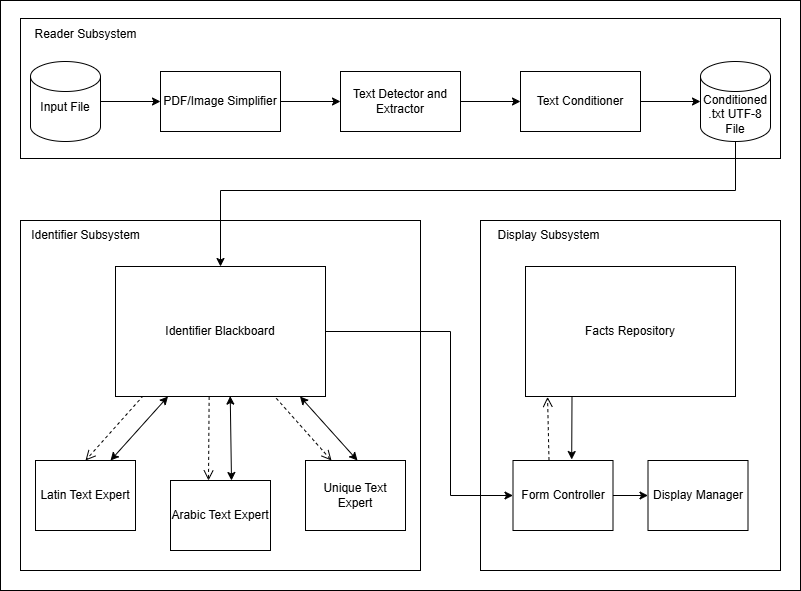
\includegraphics[width=\linewidth]{Section3/architectural_diagramV2.png}
	\caption{Architectural Diagram}
	\label{Architectural    Diagram}
\end{figure}

\begin{itemize}
    \item We considered Batch Sequential Architecture Style to transfer the data between different modules. However, using temporary files as connection between each module are not as efficient as Pipe and filter architecture which using data stream. The character of language could use ASCII table or UTF-8 to present. In this case, as long as the amount of data stream is not exceling pipe capacity, pipe could work more efficiently without waiting for temporary file from upstream.
    \item Master- Slave Architecture are also considered, since the slave nodes could implement experts of identifying the input language. However, Master-Slave Architecture features on divide the huge or data set into parts and process each part of task in parallel. And identify language is not a task that could divided in parts and send to the slave nodes. 
    \item We eliminate Model-View-Controller Architecture, through it have one data set that could store knowledge of different languages. However, the different view of displaying data is used for displaying what language we get instead of identifying languages. 
\end{itemize}

\subsection{Subsystems}
\label{sub:subsystems}
% Begin SubSection
The system’s overall functionality is facilitated by three interconnected subsystems: the Reader, Identifier, and Display services. 
\\
\\
The purpose of the Reader service is to take some form of photo, PDF, or textual language representation, and apply the necessary transformations to convert it into a plain UTF-8 text file. This behaviour is best encapsulated by a pipe and filter architecture, as the different input types dictate how they will be sequentially filtered. This can be done very efficiently over a data stream as each of the accepted file formats are static types, making them easy to binarize. Also, since users only submit a few (between 1-5) supplementary files per request, handling each one individually incurs less latency and wasted resources than using a batch sequential alternative. Data flow architectures often suffer due to their low throughputs; however, since all input processing occurs on a user’s local device, each request is managed by its own processor, and this is not an issue. These characteristics make the pipe and filter architecture ideal for the Reader service.
\\
\\
The Identifier service takes the normalized UTF-8 text provided by the Reader service, and interprets what language it is written in. To do this, it makes use of the blackboard architecture. This way, when the input arrives at the data store, it can call upon its agents (knowledge sources) to analyze the input and guess the language. More agents can be added down the line, allowing for more accurate deductions. There is no way for the agents to be certain about the language, but each offers partial solutions that build towards a comprehensive estimate. Therefore, the Identifier service’s need for an active data store and knowledge source is best fulfilled by a blackboard architecture.  
\\
\\
The third main subsystem is the Display service, which stores and returns all the interesting statistics, words, and phrases to be displayed upon language detection. As its duty is simply to store information so it can be retrieved by other agents, the repository architecture is best to implement it. The Identifier system acts as an active agent in this case by making requests for information in the passive data store. This rules out a blackboard architecture since it would need an active data store and provides uncertain partial solutions, which is not what this situation demands. The repository architecture also helps with scalability as this information is likely to be stored on a server, so when there are many concurrent requests, they all access the same network. The repository architecture is adept at handling this traffic as each one may be interpreted as a different agent, whereas a data flow architecture would have to process them one at a time, bottlenecking the system. To maintain a responsive application, the repository architecture works best for the display service. 
\\
\\
In general, the Reader service acts as a bootstrap for the blackboard identifier, and once it computes the language, the display subsystem assists it in projecting a comprehensive output to the user. 
% End SubSection